% =============================================================================
%  main.tex — DESY Test Beam Metadata Schema
%  Author : Ali Farzanehpoor Alwars  <a.farzaneh@desy.de>
%  Build  : latexmk -pdf -outdir=build main.tex   (or ./watch_build.sh)
%
%  External material
%     a.tex  — included as a source fragment, inherits report styling
%     b.pdf  — inserted verbatim as pages (pdfpages), Appendix
%     *.xsd / *.xml — pulled in with \code{lang}{file}{caption}{label}
% =============================================================================
\documentclass[11pt,a4paper]{report}

% ------------------------------------------------------------------ fonts ---
\usepackage[T1]{fontenc}
\usepackage[utf8]{inputenc}
\usepackage{amsmath,amsthm,mathtools}
\IfFileExists{libertinus.sty}
  {\usepackage{libertinus}}
  {\usepackage{lmodern}\PackageWarningNoLine{main}{libertinus missing -> lmodern}}

% --- monospace font for listings (readable, sans-style, upright) ------------
% Without this, \ttfamily falls back to Computer Modern Typewriter under
% T1 + libertinus: thin, slanted-looking, poor at small sizes.
% Optional: if inconsolata is absent the compile still succeeds.
\IfFileExists{inconsolata.sty}
  {\usepackage[varqu,varl,scaled=0.96]{inconsolata}}
  {\PackageWarningNoLine{main}{inconsolata missing -- using default monospace}}

% ------------------------------------------------------------- typography ---
\usepackage[english]{babel}
\usepackage{microtype}
\usepackage{setspace}
\setstretch{1.10}

% --------------------------------------------------------------- geometry ---
\usepackage[a4paper,
            top=2.6cm, bottom=2.6cm, left=2.8cm, right=2.8cm,
            headheight=1.4cm, headsep=0.6cm, footskip=1.2cm]{geometry}

% --------------------------------------------------------------- graphics ---
\usepackage{graphicx}
\graphicspath{{./}{./images/}}
\usepackage{float}
\usepackage{caption}
\captionsetup{font=small,labelfont=sc,labelsep=period,margin=1em}

% ------------------------------------------------- external PDF insertion ---
\usepackage{pdfpages}   % \includepdf — for b.pdf

% ----------------------------------------------------------------- tables ---
\usepackage{booktabs,array,multirow,tabularx}

% ------------------------------------------------------------------- tikz ---
\usepackage{tikz}
\usetikzlibrary{shapes,arrows.meta,positioning,calc,decorations.pathreplacing,fit,backgrounds}

% ------------------------------------------------------------------ colors ---
\usepackage{xcolor}
\definecolor{desyblue}{RGB}{0,60,120}
\definecolor{linkcolor}{RGB}{25,55,110}
\definecolor{citecolor}{RGB}{25,90,50}

% =============================================================================
%  HEADER / FOOTER — DESY logo, tunable geometry
% =============================================================================
\usepackage{fancyhdr}

% ---- 1) KNOBS: logo and header-text placement -------------------------------
% Height of the logo inside the running header. Bigger = more prominent.
\newcommand{\logoheight}{0.66cm}
% Logo offset: positive x = right, positive y = up (raisebox direction).
\newcommand{\logoXshift}{0pt}
\newcommand{\logoYshift}{-1.5pt}
% Header text offset: same convention.
\newcommand{\headtextXshift}{0pt}
\newcommand{\headtextYshift}{0.5pt}
% -----------------------------------------------------------------------------

\newcommand{\desylogo}[1]{%
  \IfFileExists{Desy_logo_3c_web.pdf}%
    {
\includegraphics[height=#1]{Desy_logo_3c_web.pdf}}%
    {\textbf{DESY}}%
}

% Marks: left header = current *section* (chapter title on a chapter's first
% page, where no section mark exists yet). Do NOT use \leftmark.
\renewcommand{\chaptermark}[1]{\markboth{}{\thechapter\quad #1}}
\renewcommand{\sectionmark}[1]{\markright{\thesection\quad #1}}

\newcommand{\desyheadrule}{%
  \renewcommand{\headrulewidth}{0.4pt}%
  \renewcommand{\headrule}{%
    \hbox to\headwidth{\color{desyblue}\leaders\hrule height \headrulewidth\hfill}}}

% Build the two header cells once, so both styles stay identical.
\newcommand{\desyheadleft}{%
  \raisebox{\headtextYshift}{\hspace*{\headtextXshift}%
    \small\nouppercase{\rightmark}}}
\newcommand{\desyheadright}{%
  \raisebox{\logoYshift}{\hspace*{\logoXshift}%
    \desylogo{\logoheight}}}

\fancypagestyle{desy}{%
  \fancyhf{}%
  \fancyhead[L]{\desyheadleft}%
  \fancyhead[R]{\desyheadright}%
  \fancyfoot[C]{\small\thepage}%
  \desyheadrule
}
\fancypagestyle{plain}{%
  \fancyhf{}%
  \fancyhead[L]{\desyheadleft}%
  \fancyhead[R]{\desyheadright}%
  \fancyfoot[C]{\small\thepage}%
  \desyheadrule
}
\pagestyle{desy}

% =============================================================================
%  CODE / LISTINGS — syntax highlighting
% =============================================================================
\usepackage{listings}

% --- palette: print-safe adaptation of VS Code Dark+ -------------------------
\definecolor{codebg}{RGB}{250,250,250}      % near-white page tint
\definecolor{codecomment}{RGB}{0,120,60}    % green
\definecolor{codestring}{RGB}{163,65,0}     % burnt orange
\definecolor{codekeyword}{RGB}{30,60,150}   % blue      (elements / tags)
\definecolor{codeattr}{RGB}{0,105,140}      % teal      (attribute names)
\definecolor{coderule}{RGB}{205,205,205}    % frame
\definecolor{codetree}{RGB}{60,60,60}       % tree glyphs

% --- generic XML -------------------------------------------------------------
\lstdefinelanguage{XML}{
  sensitive=true,
  alsoletter={:,-,_,.},
  morestring=[b]",
  morestring=[b]',
  morecomment=[s]{<!--}{-->},
  morecomment=[s]{<?}{?>},
  moredelim=[s][\color{codecomment}]{<!DOCTYPE}{>},
  moredelim=[s][\color{codecomment}]{<![CDATA[}{]]>},
  keywordstyle=[1]{\color{codekeyword}\bfseries},
}

% --- instance XML: your vocabulary, so tags are coloured too ------------------
% Extend this list as the schema grows. Keep names lowercase as in the files.
\lstdefinelanguage{MyXML}[XML]{
  morekeywords=[1]{
    run, event, payload, beamtime, device, daq, provenance,
    identifier, identifierList, status, people, role, checksum,
    storage, catalogue, access, policy, rights, licence, funding,
    references, relations, measurement, configuration
  },
  keywordstyle=[1]{\color{codekeyword}\bfseries},
}

% --- XSD: XML + curated vocabulary (elements blue, attributes teal) ----------
\lstdefinelanguage{XSD}[XML]{
  morekeywords=[1]{
    xs:schema, xs:element, xs:attribute, xs:complexType, xs:simpleType,
    xs:sequence, xs:choice, xs:all, xs:group, xs:attributeGroup,
    xs:restriction, xs:extension, xs:list, xs:union, xs:simpleContent,
    xs:complexContent, xs:annotation, xs:appinfo, xs:documentation,
    xs:include, xs:import, xs:redefine, xs:key, xs:keyref, xs:unique,
    xs:selector, xs:field, xs:enumeration, xs:pattern, xs:length,
    xs:minLength, xs:maxLength, xs:minInclusive, xs:maxInclusive,
    xs:minExclusive, xs:maxExclusive, xs:totalDigits, xs:fractionDigits,
    xs:whiteSpace, xs:any, xs:anyAttribute, xs:notation, xs:assert,
    xs:alternative, xs:openContent
  },
  morekeywords=[2]{
    name, type, ref, base, value, use, default, fixed, form, id,
    minOccurs, maxOccurs, abstract, mixed, nillable, substitutionGroup,
    targetNamespace, elementFormDefault, attributeFormDefault,
    schemaLocation, namespace, version, encoding, processContents,
    memberTypes, itemType, xpath, minVersion, maxVersion, mode, test
  },
  keywordstyle=[1]{\color{codekeyword}\bfseries},
  keywordstyle=[2]{\color{codeattr}},
}

% --- shared layout -----------------------------------------------------------
\lstset{
  basicstyle=\ttfamily\small,
  identifierstyle=\color{black!88},
  keywordstyle=\color{codekeyword}\bfseries,     % class 1
  keywordstyle=[1]{\color{codekeyword}\bfseries},
  keywordstyle=[2]{\color{codeattr}},
  stringstyle=\color{codestring},
  commentstyle=\color{codecomment}\itshape,
  backgroundcolor=\color{codebg},
  frame=single, rulecolor=\color{coderule}, framesep=4pt,
  xleftmargin=12pt, xrightmargin=0pt,
  columns=fullflexible, keepspaces=true,
  basewidth=0.5em,                               % steady monospace rhythm
  breaklines=true, breakatwhitespace=true,
  postbreak=\mbox{\textcolor{gray}{$\hookrightarrow$}\space},
  showstringspaces=false,
  tabsize=2,
  captionpos=b, aboveskip=1.2em, belowskip=0.8em,
}

% --- ASCII directory tree ----------------------------------------------------
\lstdefinestyle{tree}{
  language=,
  basicstyle=\ttfamily\small\color{codetree},
  columns=fullflexible, keepspaces=true,
  breaklines=false,
  frame=single, rulecolor=\color{coderule},
  backgroundcolor=\color{codebg},
}

% --- helper: \code{lang}{file}{caption}{label} -------------------------------
% Fails soft: a missing file yields a warning + placeholder, never a dead build.
\newcommand{\code}[4]{%
  \IfFileExists{#2}%
    {\lstinputlisting[language=#1, caption={#3}, label={lst:#4}]{#2}}%
    {\PackageWarningNoLine{main}{missing listing file: #2}%
     \begin{center}\itshape\small (#2 not available)\end{center}}%
}

% -------------------------------------------------------- section styling ---
\usepackage{titlesec}
\titleformat{\chapter}[block]
  {\normalfont\huge\bfseries\raggedright}{\thechapter\quad}{0pt}{}
\titlespacing*{\chapter}{0pt}{-1em}{2em}
\titleformat{\section}
  {\normalfont\Large\bfseries}{\thesection}{0.8em}{}
\titleformat{\subsection}
  {\normalfont\large\bfseries}{\thesubsection}{0.8em}{}

% ----------------------------------------------------------------- links ----
\usepackage[colorlinks=true,
            linkcolor=linkcolor, citecolor=citecolor, urlcolor=linkcolor,
            bookmarks=true, bookmarksopen=true,
            pdftitle={Metadata Schema for DESY Test Beam},
            pdfauthor={Ali Farzanehpoor Alwars},
            pdfsubject={DESY Test Beam -- metadata schema},
            pdfkeywords={DESY, test beam, metadata, schema}]{hyperref}

% =============================================================================
%  BUILD VERSION — yyyymmdd_hhmm_<10 random digits>
%
%  Pattern:  v20261118_1442_8392017465
%
%  Precedence:
%     1. build/version.tex, if the build system writes one
%        (contents: \newcommand{\docversion}{v...}) — lets CI or the watcher
%        pin the exact version.
%     2. otherwise: today's date + current time + ten pseudo-random digits
%        drawn at compile time with \pdfuniformdeviate (pdfTeX).
% =============================================================================
\makeatletter
\newcommand{\vpad}[1]{\ifnum#1<10 0\fi\number#1}
\newcommand{\vrandten}{%
  \ifdefined\pdfuniformdeviate
    \the\pdfuniformdeviate 10\the\pdfuniformdeviate 10\the\pdfuniformdeviate 10%
    \the\pdfuniformdeviate 10\the\pdfuniformdeviate 10\the\pdfuniformdeviate 10%
    \the\pdfuniformdeviate 10\the\pdfuniformdeviate 10\the\pdfuniformdeviate 10%
    \the\pdfuniformdeviate 10%
  \else
    \vpad{\year}\vpad{\month}\vpad{\day}\vpad{\hour}\vpad{\minute}\vpad{\second}%
  \fi}
\newcommand{\vstamp}{%
  \the\year\vpad{\month}\vpad{\day}_\vpad{\hour}\vpad{\minute}_\vrandten}
\IfFileExists{build/version.tex}
  {\input{build/version.tex}}                       % external version wins
  {\newcommand{\docversion}{v\vstamp}}
\makeatother

% =============================================================================
\begin{document}

% ------------------------------------------------------------- title page ---
\begin{titlepage}
  \thispagestyle{empty}
  \centering
  \vspace*{1.2cm}
  \desylogo{2.0cm}\par
  \vspace{0.5cm}
  {\large Deutsches Elektronen-Synchrotron DESY\par}
  \vspace{3.6cm}
  {\Huge\bfseries Metadata Schema for\\[0.4em] DESY Test Beam\par}
  \vspace{0.9cm}
  {\Large Technical Report\par}
  \vfill
  {\large Ali Farzanehpoor Alwars\par}
  \vspace{0.25cm}
  {\normalsize\href{mailto:a.farzaneh@desy.de}{\texttt{a.farzaneh@desy.de}}\par}
  \vspace{0.25cm}
  {\normalsize Version \docversion\ ---\ \today\par}
\end{titlepage}

% ------------------------------------------------------------ front matter --
\pagenumbering{roman}

\tableofcontents
\thispagestyle{plain}
\clearpage

% -------------------------------------------------------------- main matter -
\pagenumbering{arabic}

\chapter{Introduction}
\label{ch:intro}
The running header of this page shows the \emph{section} on the left and the
DESY logo on the right, both above the rule.

\section{Background}
\label{sec:background}
Test-beam data are only reusable if the acquisition conditions are recorded
in a machine-readable way.
\begin{equation}
    x = \frac{-b \pm \sqrt{b^2 - 4ac}}{2a}
    \label{eq:quadratic}
\end{equation}

\section{Scope}
\label{sec:scope}
The schema covers run, device, and beam-line metadata.

\chapter{Schema Definition}
\label{ch:schema}

\section{Entities}
\label{sec:entities}
\begin{table}[H]
    \centering
    \caption{Comparison of serialisation formats.}
    \label{tab:formats}
    \begin{tabular}{@{}lcc@{}}
        \toprule
        \textbf{Format} & \textbf{Human readable} & \textbf{Schema support} \\
        \midrule
        JSON  & yes & full \\
        YAML  & yes & full \\
        ROOT  & no  & partial \\
        \bottomrule
    \end{tabular}
\end{table}

\section{Relations}
\label{sec:relations}
\begin{figure}[H]
    \centering
    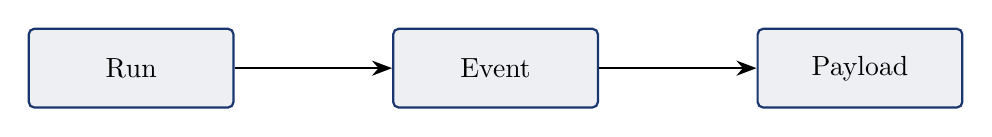
\begin{tikzpicture}[
        node distance=2cm,
        box/.style={rectangle, draw=linkcolor, fill=linkcolor!8, thick,
                    minimum width=2.6cm, minimum height=1cm,
                    align=center, rounded corners=2pt},
        arrow/.style={-{Stealth[scale=1.1]}, thick}
    ]
        \node[box] (run)     {Run};
        \node[box, right=of run]     (event)   {Event};
        \node[box, right=of event]   (payload) {Payload};
        \draw[arrow] (run)   -- (event);
        \draw[arrow] (event) -- (payload);
    \end{tikzpicture}
    \caption{Entity relations of the schema.}
    \label{fig:entities}
\end{figure}

\chapter{Conclusion}
\label{ch:conclusion}
The schema is versioned together with the report.

% =============================================================================
%  EXTERNAL MATERIAL
% =============================================================================

% --- 1) another .tex file, merged as if typed here ---------------------------
% The file must be a FRAGMENT: no \documentclass, no \begin{document}.
% Edits to a.tex trigger a rebuild (matches WATCH_REGEX \.tex$).
\IfFileExists{a.tex}{%
  % a.tex — fragment: no \documentclass, no \begin{document}
\chapter{Schema Layout}
\label{ch:layout}

The repository is organised so that core vocabulary, facility extensions and
experiment bindings can be versioned independently.

\begin{lstlisting}[style=tree, caption={Directory layout of the metadata-schema repository.},
                   label={lst:layout}]
metadata-schemas/
|
|-- core/
|   |-- identifiers-and-status
|   |-- people-and-roles
|   |-- dates-and-units
|   |-- rights-and-licences
|   |-- access-policy
|   |-- funding-and-discovery
|   |-- references-and-relations
|   |-- files-and-checksums
|   |-- storage-and-catalogues
|   |-- runs-and-measurements
|   |-- devices-and-configurations
|   |-- daq-and-control-references
|   |-- provenance
|
|-- facilities/
|   |-- testbeam/
|   |   |-- beamtime-and-slots
|   |   |-- beam-and-area
|   |   |-- diagnostics-and-safety
|   |-- other-facility/
|
|-- experiments/
|   |-- babyiaxo/
|   |-- alps2/
|   |-- madmax/
|   |-- flashforward/
|
|-- validation/
|   |-- xsd/
|   |-- shared-rules/
|   |-- facility-rules/
|   |-- experiment-rules/
|   |-- integration-tests/
|
|-- examples/
|   |-- testbeam-babyiaxo/
|   |-- alps2/
|   |-- madmax-and-flashforward/
|   |-- invalid-examples/
|
|-- migrations-and-compatibility/
|   |-- schema-versions/
|   |-- upgrade-rules/
|   |-- compatibility-tests/
|
|-- documentation/
\end{lstlisting}

The layout in Listing~\ref{lst:layout} separates concerns: \texttt{core} holds
facility-independent vocabulary, while \texttt{facilities} and
\texttt{experiments} extend it without forking.
%
}{%
  \PackageWarningNoLine{main}{a.tex not found -- skipping}%
}

% --- 2) schema sources pulled in as listings --------------------------------
\chapter{Core Schema Files}
\label{ch:schemas}

\section{Identifiers and status}
\label{sec:identifiers}
The identifier block is defined in \texttt{core/identifiers.xsd}:
\code{XSD}{core/identifiers.xsd}{Definition of identifier and status types.}{identifiers}

A conforming instance looks like this:
\code{MyXML}{examples/testbeam-babyiaxo/run-0001.xml}{Example run document.}{run0001}

% --- 3) an external PDF, inserted page-for-page, as an appendix ------------
\IfFileExists{b.pdf}{%
  \clearpage
  \appendix
  \chapter{External Document}
  \label{app:external}
  \includepdf[
      pages=-,                             % - = all pages; also 1-3, 5, 7-
      pagecommand={\thispagestyle{desy}},  % DESY header over each page
      fitpaper=false,                      % true = use source page size
      scale=0.94,                          % shrink to fit the text block
      offset=0 -0.6cm,                     % nudge vertically if needed
      frame=false,                         % true = thin border, for checks
      link=false,                          % no hyperlinks from the source
  ]{b.pdf}%
  \clearpage
}{%
  \PackageWarningNoLine{main}{b.pdf not found -- skipping}%
}

% ------------------------------------------------------------- bibliography -
\IfFileExists{references.bib}{%
  \bibliographystyle{plain}%
  \bibliography{references}%
}{}

\end{document}
